\onehalfspacing
\section{Đề số 37}

\begin{bt} 
	\hfill
	\begin{enumerate}[a.]
		\item Tính giá trị biểu thức $\mathrm{P}=\left|a-\frac{1}{2014}\right|+\left|a-\frac{1}{2016}\right|$, với $a=\frac{1}{2015}$.
		\item Tìm số nguyên $\mathrm{x}$ để tích hai phân số $\frac{6}{x+1}$ và $\frac{x-1}{3}$ là một số nguyên.
	\end{enumerate}
	\loigiai{
		\begin{enumerate}
			\item Tính giá trị biểu thức $\mathrm{P}=\left|a-\frac{1}{2014}\right|+\left|a-\frac{1}{2016}\right|$, với $a=\frac{1}{2015}$.\\[5px]
			Thay $a=\frac{1}{2015}$ vào biểu thức $P=\left|\frac{1}{2015}-\frac{1}{2014}\right|+\left|\frac{1}{2015}-\frac{1}{2016}\right|$\\[5px]
			Ta có $P=\frac{1}{2014}-\frac{1}{2015}+\frac{1}{2015}-\frac{1}{2016}$\\[5px]
			$P=\frac{1}{2014}-\frac{1}{2016} \\[5px]
			P=\frac{2016-2014}{2014.2016}=\frac{2}{2014.2016} \\[5px]
			P=\frac{1}{1007.2016}=\frac{1}{2030112}$
			\item Tìm số nguyên $x$ để tích hai phân số $\frac{6}{x+1}$ và $\frac{x-1}{3}$ là một số nguyên.\\[5px]
			$\text {Đặt } \mathrm{A}=\frac{6}{x+1} \cdot \frac{x-1}{3}=\frac{2}{x+1} \cdot \frac{x-1}{1} \\[5px]
			=\frac{2(x-1)}{x+1} \\[5px]
			=\frac{2 x-2}{x+1} \\[5px]
			=\frac{2(x+1)-4}{x+1} \\[5px]
			=2-\frac{4}{x+1}$\\[5px]
			Để A nhận giá trị nguyên thì $x+1$ là Ư$(4)=\{ \pm 1 ; \pm 2 ; \pm 4\}$\\[5px]
			Suy ra x $\in\{0 ;-2 ; 1 ;-3 ; 3 ;-5\}$
		\end{enumerate}
	} 
\end{bt}

\begin{bt}
	\hfill
	\begin{enumerate}[a.]
		\item Cho $\mathrm{a}>2, \mathrm{~b}>2$. Chứng minh $a b>a+b$
		\item Cho ba hình chữ nhật, biết diện tích của hình thứ nhất và diện tích của hình thứ hai tỉ lệ với 4 và 5 , diện tích hình thứ hai và diện tích hình thứ ba tỉ lệ với 7 và 8 , hình thứ nhất và hình thứ hai có cùng chiều dài và tổng các chiều rộng của chúng là $27 \mathrm{~cm}$, hình thứ hai và hình thứ ba có cùng chiều rộng, chiều dài của hình thứ ba là $24 \mathrm{~cm}$. Tính diện tích của mỗi hình chữ nhật đó.
	\end{enumerate}
	\loigiai{
		\begin{enumerate}
			\item Cho $\mathrm{a}>2, \mathrm{~b}>2$. Chứng minh $a b>a+b$\\[5px]
			Từ $a>2 \Rightarrow \frac{1}{a}<\frac{1}{2}$
			$b>2 \Rightarrow \frac{1}{b}<\frac{1}{2}$\\[5px]
			Suy ra $\frac{1}{a}+\frac{1}{b}<1 \Rightarrow \frac{a+b}{a b}<1$\\[5px] 
			Vậy $ab> a + b$
			\item Gọi diện tích ba hình chữ nhật lần lượt là $S_1, S_2, S_3$, chiều dài, chiều rộng tương ứng là $d_1, r_1 ; d_2, r_2 ; d_3, r_3$ theo đề bài ta có:\\[5px]
			$\frac{S_1}{S_2}=\frac{4}{5} ; \frac{S_2}{S_3}=\frac{7}{8} \text { và } d_1=d_2 ; r_1+r_2=27 ; r_2=r_3, d_3=24$\\[5px]
			Vì hình thứ nhất và hình thứ hai cùng chiều dài\\[5px]
			$\frac{S_1}{S_2}=\frac{4}{5}=\frac{r_1}{r_2} \Rightarrow \frac{r_1}{4}=\frac{r_2}{5}=\frac{r_1+r_2}{9}=\frac{27}{9}=3$\\[5px]
			Suy ra chiều rộng $r_1=12 \mathrm{~cm}, r_2=15 \mathrm{~cm}$\\[5px]
			Vì hình thứ hai và hình thứ ba cùng chiều rộng\\[5px]
			$\frac{S_2}{S_3}=\frac{7}{8}=\frac{d_2}{d_3} \Rightarrow d_2=\frac{7 d_3}{8}=\frac{7.24}{8}=21 \mathrm{~cm}$\\[5px]
			Vậy diện tích hình thứ hai $S_2=d_2 r_2=21.15=315 \mathrm{~cm}^2$\\[5px]
			Diện tích hình thứ nhất:\\[5px]
			$S_1=\frac{4}{5} S_2=\frac{4}{5} \cdot 315=252 \mathrm{~cm}^2$\\[5px]
			Diện tích hình thứ ba: $S_3=\frac{8}{7} S_2=\frac{8}{7} \cdot 315=360 \mathrm{~cm}^2$
		\end{enumerate}
	} 
\end{bt}

\begin{bt}
	Cho tam giác $A B C, M$ là trung điểm của $B C$. Trên tia đối của tia MA lấy điểm $E$ sao cho $\mathrm{ME}=\mathrm{MA}$. Chứng minh rằng:
	\begin{enumerate}[a.]
		\item AC = EB và AC // BE
		\item Gọi I là một điểm trên $\mathrm{AC}, \mathrm{K}$ là một điểm trên $\mathrm{EB}$ sao cho: $\mathrm{AI}=\mathrm{EK}$. Chứng minh: $\mathrm{I}, \mathrm{M}, \mathrm{K}$ thẳng hàng.
		\item Từ $\mathrm{E}$ kẻ $\mathrm{EH} \perp \mathrm{BC}(\mathrm{H} \in \mathrm{BC})$. Biết góc $\mathrm{HBE}$ bằng $50^{\circ}$; góc $\mathrm{MEB}$ bằng $25^{\circ}$, tính các góc $H E M$ và $B M E$ ?
	\end{enumerate}
	\loigiai{
		$$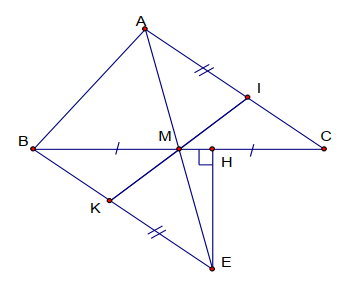
\includegraphics[width=0.5\textwidth]{37-3-lg.png}$$
		\begin{enumerate}
			\item Xét $\triangle A M C$ và $\triangle E M B$ có:\\[5px]
			$\mathrm{AM}=\mathrm{EM} \quad(\mathrm{gt}) \\[5px]
			A M C=E M B \quad \text { (đối đỉnh }) \\[5px]
			\mathrm{BM}=\mathrm{MC} \quad(\mathrm{gt}) \\[5px]
			\text {Nên : } \triangle A M C=\triangle E M B \quad \text { (c.g.c ) } \\[5px]
			\Rightarrow \mathrm{AC}=\mathrm{EB} \\[5px]
			\text {Vì } \triangle A M C=\triangle E M B \\[5px]
			\Rightarrow \text {Góc MAC bằng góc } \mathrm{MEB}$\\[5px]
			(2 góc có vị trí so le trong được tạo bởi đường thẳng $\mathrm{AC}$ và $\mathrm{EB}$ cắt đường thẳng $\mathrm{AE}$ ).\\[5px] 
			Suy ra $A C / / \mathrm{BE}$.
			\item Xét $\triangle A M I$ và $\triangle E M K$ có:\\[5px] 
			$\mathrm{AM}=\mathrm{EM}(\mathrm{gt}) \\[5px]
			M A I=M E K(\text { vì } \triangle A M C=\triangle E M B) \\[5px]
			\mathrm{AI}=\mathrm{EK}(\mathrm{gt})$\\[5px]
			Nên $\triangle A M I=\Delta E M K$ ( c.g.c ). Suy ra $A M I=E M K$\\[5px]
			Mà $A M I+I M E=180^{\circ}$ ( tính chất hai góc kề bù )\\[5px]
			$\Rightarrow \mathrm{EMK}+I \mathrm{ME}=180^{\circ} \Rightarrow \mathrm{Ba}$ điểm $\mathrm{I} ; \mathrm{M} ; \mathrm{K}$ thẳng hàng\\[5px]
			\item Trong tam giác vuông BHE ( $\left.H=90^{\circ}\right)$ có $H B E=50^{\circ}$\\[5px]
			$\Rightarrow H B E=90^{\circ}-H B E=90^{\circ}-50^{\circ}=40^{\circ} \\[5px]
			\Rightarrow H E M=H E B-M E B=40^{\circ}-25^{\circ}=15^{\circ}$\\[5px]
			$B M E$ là góc ngoài tại đỉnh $\mathrm{M}$ của $\triangle H E M$\\[5px]
			Nên $B M E=H E M+M H E=15^{\circ}+90^{\circ}=105^{\circ}$( định lý góc ngoài của tam giác )
		\end{enumerate}
	}
\end{bt}

\begin{bt}
	Cho các số $0<a_1<a_2<a_3<\ldots . .<a_{15}$. Chứng minh rằng $\frac{a_1+a_2+a_3+\ldots+a_{15}}{a_5+a_{10}+a_{15}}<5$
	\loigiai{
		Cho các số $0<a_1<a_2<a_3<\ldots<a_{15}$.\\[5px]
		Chứng minh rằng $\frac{a_1+a_2+a_3+\ldots+a_{15}}{a_5+a_{10}+a_{15}}<5$\\[5px]
		Ta có $a_1+a_2+a_3+a_4+a_5<5 a_5$\\[5px]
		$a_6+a_7+a_8+a_9+a_{10}<5 a_{10} \\[5px]
		a_{11}+a_{12}+a_{13}+a_{14}+a_{15}<5 a_{15}$\\[5px]
		Suy ra $a_1+a_2+\ldots \ldots . .+a_{15}<5\left(a_5+a_{10}+a_{15}\right)$\\[5px]
		Vậy $\frac{a_1+a_2+a_3+\ldots+a_{15}}{a_5+a_{10}+a_{15}}<5$
	}
\end{bt}

\begin{bt}
	Cho $\triangle \mathrm{ABC}$ nhọn với $B A C=60^{\circ}$. Chứng minh rằng:
	$$
	\mathrm{BC}^2=\mathrm{AB}^2+\mathrm{AC}^2-\mathrm{AB} \cdot \mathrm{AC}
	$$
	\loigiai{
		$$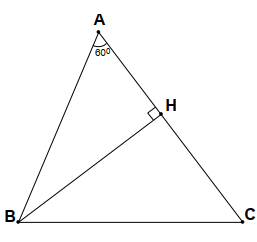
\includegraphics[width=0.35\textwidth]{37-5-lg.png}$$
		Kẻ $\mathrm{BH} \perp \mathrm{AC}$\\[5px]
		Vì $B A C=60^{\circ} \Rightarrow A B H=30^{\circ} \Rightarrow A H=\frac{A B}{2}$ (1)\\[5px]
		Áp dụng định lý Pitago ta có:\\[5px]
		$\mathrm{AB}^2=\mathrm{AH}^2+\mathrm{BH}^2 \text { và } \mathrm{BC}^2=\mathrm{BH}^2+\mathrm{HC}^2 \Rightarrow \mathrm{BC}^2=\mathrm{AB}^2-\mathrm{AH}^2+\mathrm{HC}^2 \\[5px]
		\Rightarrow \mathrm{BC}^2=\mathrm{AB}^2-\mathrm{AH}^2+(\mathrm{AC}-\mathrm{AH})^2 \Rightarrow \mathrm{BC}^2=\mathrm{AB}^2-\mathrm{AH}^2+\mathrm{AC}^2-2 \mathrm{AC} \cdot \mathrm{AH}+\mathrm{AH}^2 \\[5px]
		\Rightarrow \mathrm{BC}^2=\mathrm{AB}^2+\mathrm{AC}^2-2 \mathrm{AC} \cdot \mathrm{AH}(2) \\[5px]
		\text {Từ (1) \& (2) } \Rightarrow \text { đpcm }$
	} 
\end{bt}